\documentclass[tikz,border=2pt]{standalone}
\usepackage{amsmath}
\usepackage{pgfplots}
\pgfplotsset{compat=1.18}
\usetikzlibrary{arrows.meta}
\begin{document}
% A(t)/t for inter-arrival times alternating 1,3 (arrivals 1,4,5,8,9,...): on [A_k, A_{k+1}) the ratio is k/t;
% the values k/A_k at arrivals (dots) and the troughs both tend to lambda = 1/2 = 1/E[X].
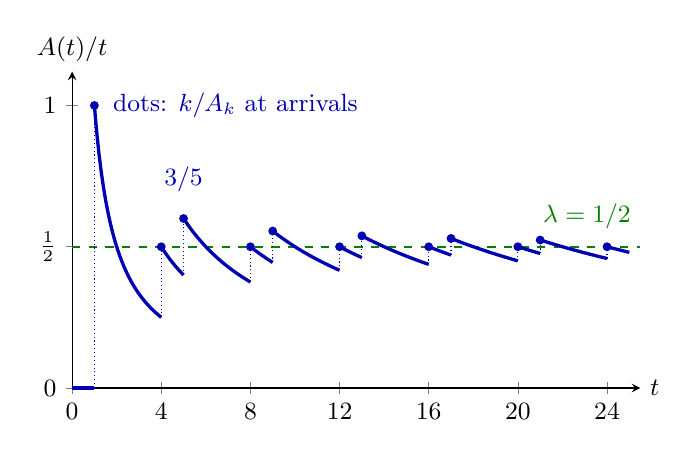
\begin{tikzpicture}[font=\small, >={Latex[length=2mm]}]
  \begin{axis}[
    axis lines=left, xmin=0, xmax=25.5, ymin=0, ymax=1.12,
    xtick={0,4,8,12,16,20,24}, ytick={0,0.5,1},
    yticklabels={$0$,$\tfrac{1}{2}$,$1$},
    xlabel={$t$}, ylabel={$A(t)/t$},
    xlabel style={at={(axis description cs:1,0)}, anchor=west},
    ylabel style={rotate=-90, at={(axis description cs:0,1)}, anchor=south},
    width=8.8cm, height=5.6cm, clip=false
    ]
    \draw[green!50!black, thick, dashed] (axis cs:0,0.5) -- (axis cs:25.5,0.5);
    \node[green!50!black, anchor=south east] at (axis cs:25.5,0.53) {$\lambda=1/2$};
    \draw[blue!70!black, very thick] (axis cs:0,0) -- (axis cs:1,0);
    \draw[blue!70!black, thin, densely dotted] (axis cs:1,0.0000) -- (axis cs:1,1.0000);
    \draw[blue!70!black, thin, densely dotted] (axis cs:4,0.2500) -- (axis cs:4,0.5000);
    \draw[blue!70!black, thin, densely dotted] (axis cs:5,0.4000) -- (axis cs:5,0.6000);
    \draw[blue!70!black, thin, densely dotted] (axis cs:8,0.3750) -- (axis cs:8,0.5000);
    \draw[blue!70!black, thin, densely dotted] (axis cs:9,0.4444) -- (axis cs:9,0.5556);
    \draw[blue!70!black, thin, densely dotted] (axis cs:12,0.4167) -- (axis cs:12,0.5000);
    \draw[blue!70!black, thin, densely dotted] (axis cs:13,0.4615) -- (axis cs:13,0.5385);
    \draw[blue!70!black, thin, densely dotted] (axis cs:16,0.4375) -- (axis cs:16,0.5000);
    \draw[blue!70!black, thin, densely dotted] (axis cs:17,0.4706) -- (axis cs:17,0.5294);
    \draw[blue!70!black, thin, densely dotted] (axis cs:20,0.4500) -- (axis cs:20,0.5000);
    \draw[blue!70!black, thin, densely dotted] (axis cs:21,0.4762) -- (axis cs:21,0.5238);
    \draw[blue!70!black, thin, densely dotted] (axis cs:24,0.4583) -- (axis cs:24,0.5000);
    \addplot[blue!70!black, very thick, domain=1:4, samples=30] {1/x};
    \addplot[blue!70!black, very thick, domain=4:5, samples=30] {2/x};
    \addplot[blue!70!black, very thick, domain=5:8, samples=30] {3/x};
    \addplot[blue!70!black, very thick, domain=8:9, samples=30] {4/x};
    \addplot[blue!70!black, very thick, domain=9:12, samples=30] {5/x};
    \addplot[blue!70!black, very thick, domain=12:13, samples=30] {6/x};
    \addplot[blue!70!black, very thick, domain=13:16, samples=30] {7/x};
    \addplot[blue!70!black, very thick, domain=16:17, samples=30] {8/x};
    \addplot[blue!70!black, very thick, domain=17:20, samples=30] {9/x};
    \addplot[blue!70!black, very thick, domain=20:21, samples=30] {10/x};
    \addplot[blue!70!black, very thick, domain=21:24, samples=30] {11/x};
    \addplot[blue!70!black, very thick, domain=24:25, samples=30] {12/x};
    \fill[blue!70!black] (axis cs:1,1.0000) circle (1.6pt);
    \fill[blue!70!black] (axis cs:4,0.5000) circle (1.6pt);
    \fill[blue!70!black] (axis cs:5,0.6000) circle (1.6pt);
    \fill[blue!70!black] (axis cs:8,0.5000) circle (1.6pt);
    \fill[blue!70!black] (axis cs:9,0.5556) circle (1.6pt);
    \fill[blue!70!black] (axis cs:12,0.5000) circle (1.6pt);
    \fill[blue!70!black] (axis cs:13,0.5385) circle (1.6pt);
    \fill[blue!70!black] (axis cs:16,0.5000) circle (1.6pt);
    \fill[blue!70!black] (axis cs:17,0.5294) circle (1.6pt);
    \fill[blue!70!black] (axis cs:20,0.5000) circle (1.6pt);
    \fill[blue!70!black] (axis cs:21,0.5238) circle (1.6pt);
    \fill[blue!70!black] (axis cs:24,0.5000) circle (1.6pt);
    \node[blue!70!black, anchor=west] at (axis cs:1.4,1.0) {dots: $k/A_k$ at arrivals};
    \node[blue!70!black, anchor=south] at (axis cs:5,0.66) {$3/5$};
  \end{axis}
\end{tikzpicture}
\end{document}
